% Contenidos del capítulo.
% Las secciones presentadas son orientativas y no representan
% necesariamente la organización que debe tener este capítulo.

% Introducción
En el presente capítulo se lleva a cabo un análisis del estado del arte con el fin de situar el 
proyecto en el contexto de soluciones existentes y tecnologías actuales. La plataforma 
web desarrollada en este \gls{tfg} tiene como objetivo facilitar el emparejamiento entre 
profesionales y proyectos mediante un sistema basado en competencias jerarquizadas. 
Por ello, resulta esencial estudiar qué herramientas similares existen ya en el mercado 
y cómo se enfrentan a problemas de emparejamiento, recomendación o gestión de 
talento y proyectos.

Primero se presentarán aplicaciones con funcionalidades relacionadas, analizando sus 
características principales, puntos en común con esta propuesta y diferencias clave. 
Este estudio permitirá identificar tanto aspectos que se consideran imprescindibles en 
una plataforma de este tipo, como oportunidades de mejora o innovación.

Posteriormente se realizará un análisis crítico de las tecnologías más relevantes para el 
desarrollo del sistema, justificando la elección final en cada caso a partir de criterios 
como la escalabilidad, facilidad de desarrollo, mantenimiento o compatibilidad entre 
componentes.

Por último, se listarán aquellas herramientas de soporte utilizadas durante el desarrollo 
del \gls{tfg}, como entornos de desarrollo, sistemas de control de versiones o editores 
de diagramas, las cuales han sido fundamentales para llevar a cabo el proyecto.

% 2.1
\section{Análisis de aplicaciones similares}
% Qué aplicaciones similares hay y en qué se diferencia de ellas la propuesta
En esta sección se analizarán distintas aplicaciones existentes que presentan elementos 
comunes con la \textbf{plataforma web desarrollada en este trabajo}, cuyo objetivo es 
facilitar el \textbf{emparejamiento entre profesionales y proyectos} en función de sus 
competencias. Para ello, se comentarán \textbf{soluciones reales} que abordan problemas 
similares, ya sea desde la perspectiva de \textbf{plataformas orientadas al empleo y el talento}, 
o desde el enfoque de \textbf{sistemas de emparejamiento inteligente basados en afinidad}.

Dado que el proyecto combina ideas presentes en entornos profesionales como LinkedIn \cite{linkedin}
y en algoritmos de emparejamiento como los utilizados por aplicaciones tipo Tinder \cite{tinder}, se 
ha optado por dividir este análisis en \textbf{dos bloques diferenciados}. En el primero se 
estudiarán \textbf{plataformas centradas en la gestión del talento y la búsqueda de empleo}, 
mientras que en el segundo se abordarán \textbf{sistemas cuyo núcleo es el emparejamiento 
basado en coincidencias}, con el objetivo de extraer ideas aplicables al 
\gls{recomendaciones} que se desea implementar.

Este análisis permitirá no solo \textbf{identificar funcionalidades clave y enfoques existentes}, 
sino también detectar \textbf{carencias o posibles áreas de mejora}, con el fin de proponer 
una solución más \textbf{adaptada, automatizada} y centrada en la 
\textbf{coincidencia de competencias concretas}.

% 2.1.1
\subsection{Plataformas web orientadas al empleo y la gestión del talento}

Dado que la plataforma web a desarrollar tiene como objetivo conectar profesionales con 
proyectos en función de sus competencias, las primeras aplicaciones a analizar son aquellas 
centradas en la búsqueda de empleo, la exposición del perfil profesional y la gestión del talento.

En esta sección se analizarán concretamente las plataformas \textbf{LinkedIn} \cite{linkedin}, 
\textbf{InfoJobs} \cite{infojobs} y \textbf{Yobalia} \cite{yobalia}, destacando sus funcionalidades principales y su grado 
de similitud con la solución propuesta en este trabajo.

% LinkedIn
\subsubsection{LinkedIn}

En primer lugar, \textbf{LinkedIn} \cite{linkedin} es una plataforma web orientada al entorno 
profesional que permite a los usuarios crear un perfil con información detallada sobre su 
experiencia laboral, formación académica, certificaciones y competencias. Su objetivo 
principal es facilitar la conexión entre profesionales, empresas y oportunidades laborales, 
actuando como red social y como herramienta para la búsqueda de empleo.

Entre sus funcionalidades destaca un sistema de filtrado de ofertas que permite ajustar la 
búsqueda según múltiples parámetros, como ubicación, modalidad de trabajo (presencial o 
remoto), tipo de contrato o experiencia requerida. En la Figura \ref{fig:linkedin-ofertas} se muestra un ejemplo de 
búsqueda activa de empleo, donde se visualizan las ofertas disponibles y una vista previa de 
cada una de ellas. En particular, se ha realizado una búsqueda real orientada al perfil de 
\textbf{programador \gls{fullstack}} en la zona de \textbf{Valencia}, comprobando que la 
plataforma devuelve resultados actualizados y relevantes. Esta funcionalidad se basa en un 
sistema de filtrado tradicional implementado sobre formularios dinámicos en el 
\gls{frontend}, que construyen consultas específicas para recuperar ofertas desde su 
\gls{backend}.

Además, LinkedIn ofrece la posibilidad de añadir \textit{habilidades} al perfil de usuario, 
las cuales pueden ser validadas por otros contactos, y que posteriormente pueden ser 
utilizadas por los reclutadores para filtrar candidatos en función de sus aptitudes. 
En la Figura \ref{fig:linkedin-aptitudes} se ilustra esta sección del perfil. A pesar de ello, la plataforma no 
implementa un sistema de recomendaciones basado en coincidencias automáticas entre 
el perfil y las ofertas, sino que es el propio usuario quien debe llevar a cabo la búsqueda 
activa.

LinkedIn también dispone de herramientas de suscripción premium, que permiten acceder a 
estadísticas avanzadas sobre las postulaciones o enviar mensajes directos a reclutadores. 
Sin embargo, para el uso básico, la mayoría de funcionalidades son gratuitas.

En definitiva, LinkedIn representa un referente consolidado en la búsqueda de empleo y la 
gestión del talento, pero su funcionamiento está centrado en la exploración manual y el 
uso de filtros, sin un sistema automatizado de emparejamiento como el que se plantea en 
este trabajo.

\begin{figure}[H]
    \centering
    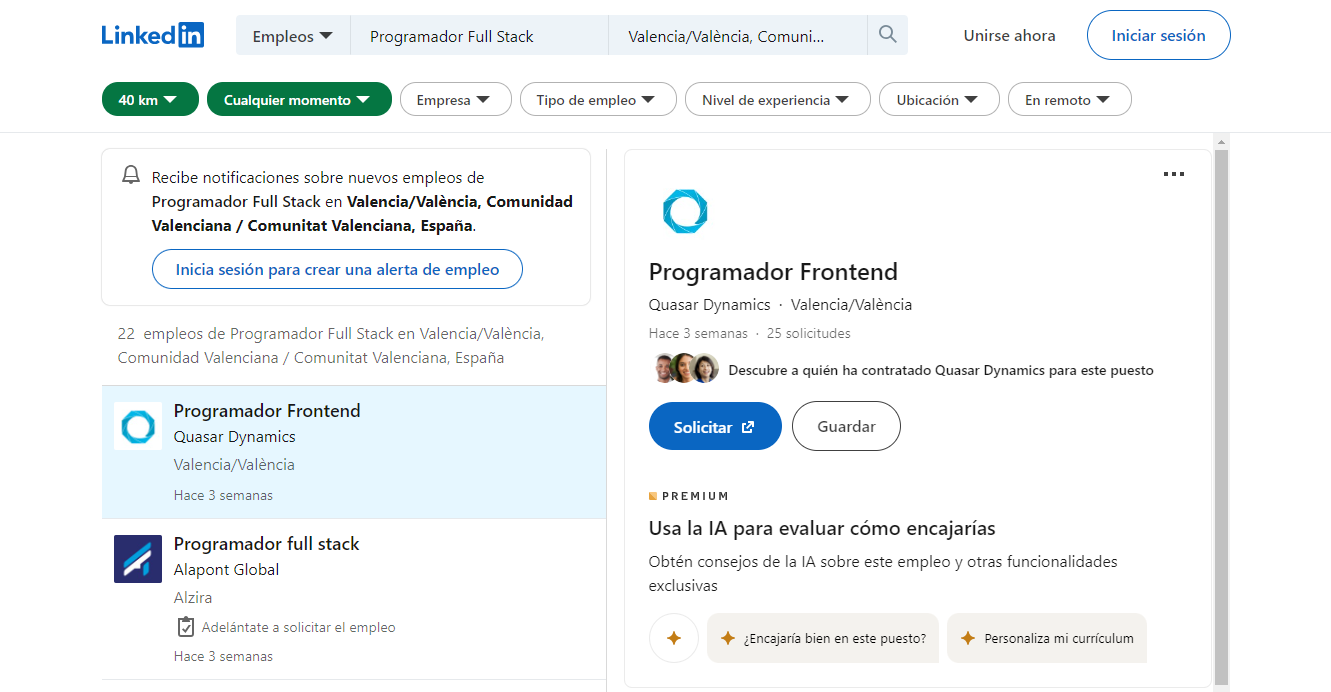
\includegraphics[width=0.9\textwidth]{figs/linkedin-ofertas.png}
    \caption{Interfaz de búsqueda de empleo en LinkedIn para ``Programador Full Stack''.}
    \label{fig:linkedin-ofertas}
  \end{figure}
  
\begin{figure}[H]
    \centering
    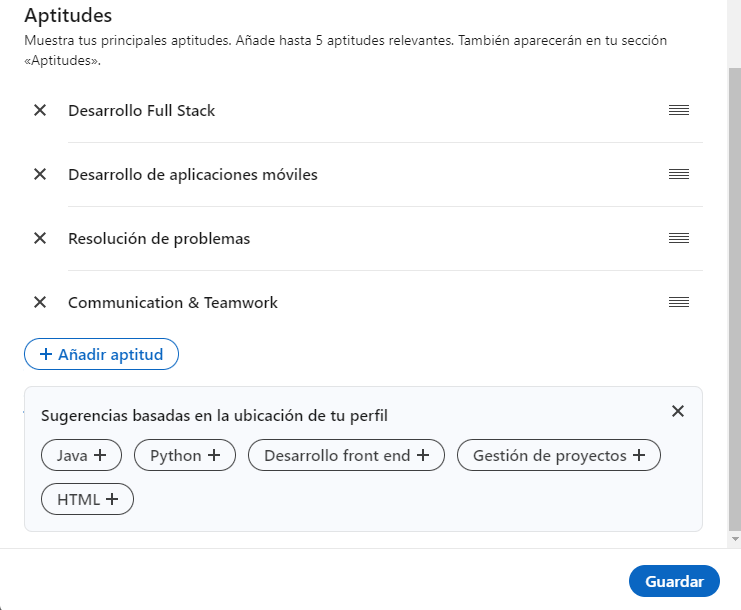
\includegraphics[width=0.65\textwidth]{figs/linkedin-aptitudes.png}
    \caption{Ejemplo de selección de aptitudes en el perfil de usuario de LinkedIn.}
    \label{fig:linkedin-aptitudes}
\end{figure}

% InfoJobs
\subsubsection{InfoJobs}

\textbf{InfoJobs} \cite{infojobs} es una plataforma generalista de búsqueda de empleo en España, 
orientada a la publicación y gestión de ofertas laborales de múltiples sectores. A diferencia de 
\textbf{LinkedIn}, su funcionamiento se centra en la inscripción directa del usuario a las ofertas, sin 
red de contactos ni validación de aptitudes.

Este sistema de búsqueda utiliza formularios predefinidos en el frontend para generar filtros 
que se aplican sobre la base de datos mediante consultas directas al backend, priorizando 
coincidencias exactas entre los criterios seleccionados y los campos del perfil del usuario. 
Sin embargo, no emplea ningún tipo de lógica avanzada de emparejamiento automático o inferencia 
basada en competencias.

En la Figura~\ref{fig:infojobs-oferta} se muestra un ejemplo de oferta publicada para un puesto de 
programador web, donde se observan los detalles del puesto, los requisitos y las opciones de inscripción.

Frente a este enfoque, la plataforma propuesta en este \gls{tfg} plantea un sistema de recomendaciones 
que busca automatizar el emparejamiento, priorizando aquellas coincidencias más relevantes entre 
las competencias del profesional y las necesidades del proyecto.

\begin{figure}[H]
    \centering
    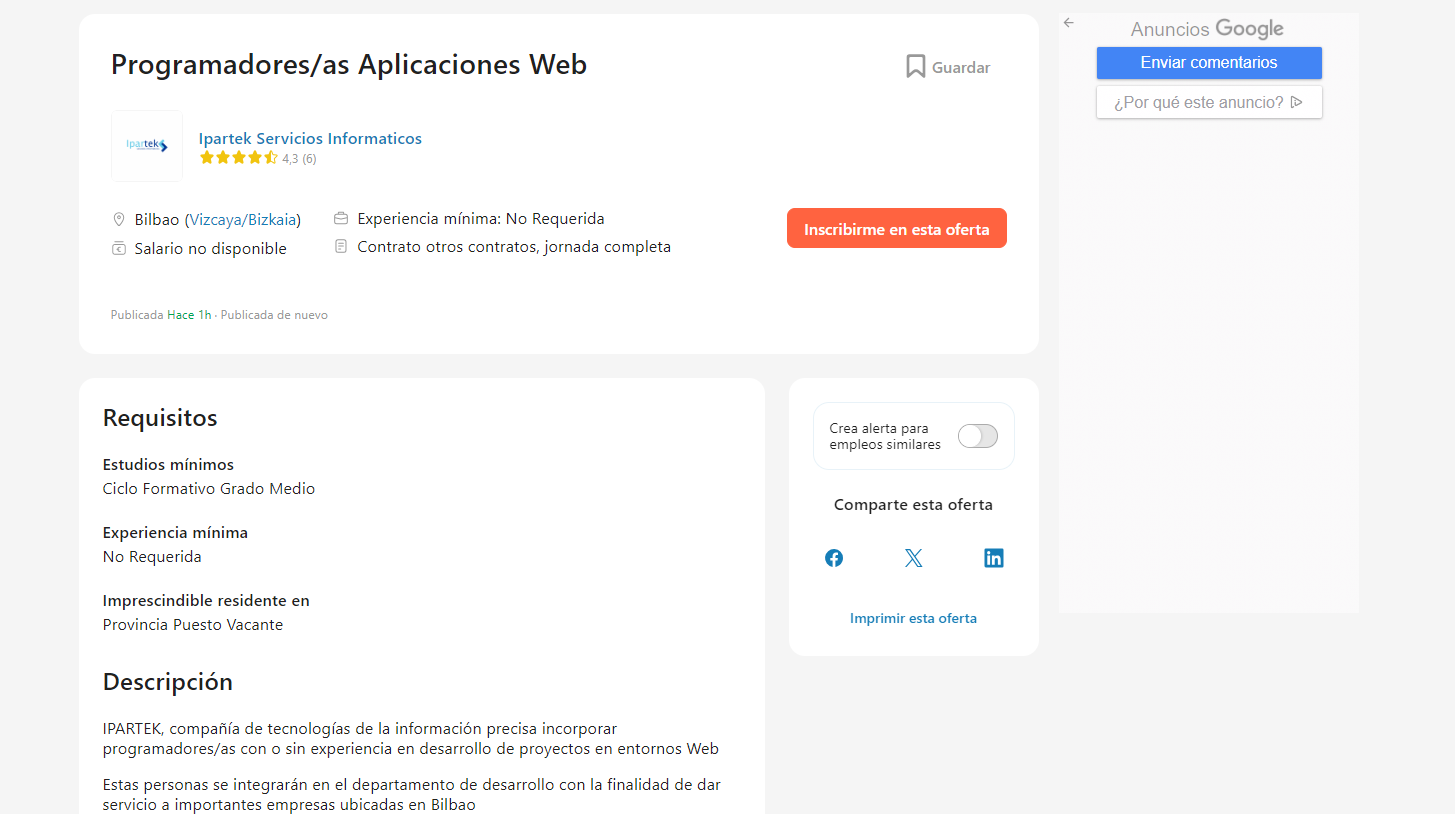
\includegraphics[width=0.85\textwidth]{figs/infojobs-oferta.png}
    \caption{Ejemplo de oferta de trabajo publicada en InfoJobs.}
    \label{fig:infojobs-oferta}
\end{figure}

% Yobalia
\subsubsection{Yobalia}

Por último, \textbf{Yobalia} \cite{yobalia} es una plataforma web de búsqueda de empleo especializada en 
el sector de eventos, promociones y acciones publicitarias. Está orientada principalmente a perfiles como 
azafatas, promotores, animadores o personal para campañas de marketing en punto de venta.

Desde su página principal queda patente esta orientación, posicionándose como un portal de referencia 
para trabajos puntuales y de corta duración. En la Figura \ref{fig:yobalia-portada} se muestra su interfaz 
de búsqueda, donde es posible filtrar las ofertas disponibles mediante criterios básicos como la ubicación, 
la categoría profesional o palabras clave introducidas por el usuario. Este último elemento guarda cierta 
relación con el sistema basado en competencias que plantea la solución de este \gls{tfg}, si bien su 
funcionamiento se basa en una coincidencia textual directa sin ningún tipo de análisis semántico o ponderación.

Aunque permite registrar el currículum y aplicar de forma rápida a las ofertas, la plataforma carece de 
validación de habilidades, conexión entre perfiles o mecanismos automatizados de emparejamiento. Todo el 
proceso de búsqueda y postulación depende de la acción manual del usuario.

En este sentido, la plataforma propuesta en este trabajo no solo abarca perfiles técnicos, sino que también 
está concebida para facilitar el acceso a trabajos eventuales como los ofrecidos en Yobalia, mejorando la 
eficiencia del proceso mediante un sistema de recomendaciones que prioriza las coincidencias entre requisitos 
y competencias de forma más automatizada.

\begin{figure}[H]
    \centering
    
\includegraphics[width=0.85\textwidth]{figs/yobalia-portada.png}
    \caption{Interfaz principal de búsqueda de empleo en Yobalia, con filtros por ubicación, categoría y palabras clave.}
    \label{fig:yobalia-portada}
\end{figure}

% Conclusiones
\subsubsection{Conclusiones}

Tras analizar las plataformas presentadas, podría cuestionarse si hubiera sido más
eficiente utilizar directamente alguna de ellas para gestionar el emparejamiento entre
profesionales y proyectos. Sin embargo, existen motivos claros para optar por una
plataforma desarrollada a medida.

\textbf{LinkedIn}, aunque potente, es una red generalista donde el emparejamiento entre
usuarios y ofertas no se basa en un sistema automático guiado por competencias, sino en
la búsqueda activa y manual. \textbf{InfoJobs}, por su parte, se basa en filtros simples
definidos por las ofertas, sin aplicar lógica de emparejamiento basada en competencias
reales. Finalmente, \textbf{Yobalia} está centrada en trabajos puntuales y carece de un
sistema de recomendación avanzado.

Por tanto, desarrollar una solución propia permite construir un modelo centrado en
competencias, adaptable a distintos tipos de perfiles y proyectos, y con capacidad de
evolución. Esta decisión garantiza una mayor flexibilidad y un control total sobre la
funcionalidad y el enfoque del sistema, ajustándose plenamente a los objetivos de este
\gls{tfg}.

% 2.1.2
\subsection{Aplicaciones con sistemas de emparejamiento basados en coincidencias}


\section{Evaluación de tecnologías}\label{sec:evaluacion-tecnologias}
% Análisis crítico de las tecnologías y sistemas de despliegue posibles y por qué se han seleccionado unas concretas.
